%   Modelo de trabalhos acadêmicos - IFRJ
%   Autor: Andrey Dione Ferreira - <andrey.ferreira@ifrj.edu.br>
%   Codificação utilizada: UTF-8
%   Tamanho da tabulação: 4 (espaços)
%	Atualizado em 01/06/2023

% \documentclass{ifrjtex}  % Imprimir frente e verso
\documentclass[oneside]{ifrjtex}  % Imprimir apenas frente

%----------------------------
% IMPORTAÇÃO DE PACOTES %
%-----------------------------

% \usepackage{smartdiagram} %Construção de diagramas
% \usepackage[portuguese, onelanguage, lined, boxed, commentsnumbered, algoruled]{algorithm2e} % Escrever algoritmos
% \usepackage{animate,pgfplots,multido} % Desenhar e fazer animações
% \pgfplotsset{compat=1.16}
\usepackage{verbatim}     % Texto é interpretado como escrito no documento
\usepackage{multirow, array}    % Múltiplas linhas e colunas em tabelas
% \usepackage{listings} % para impressão de códigos
\usepackage{pdfpages} % para inserção de página em pdf


%----
%referências bibliográficas tratadas com biblatex
\addbibresource{refbase.bib} % base bibliográfica

% Criando novos comandos ou redefinindo outros
\renewcommand{\sin}{\mathrm{sen}}

\makeindex % Cria o índice remissivo

%----------------------------------------------
% PREENCHER COM OS DADOS DO TRABALHO            
%----------------------------------------------
\titulo{Título do trabalho}
\subtitulo{Subtítulo do trabalho}
\autor{Nome Completo do Autor}
\local{Volta Redonda}
\data{Janeiro de 2016}  % coloque a data de defesa no formato Mês de Ano
\instituicao{Instituto Federal de Educação, Ciência e Tecnologia do Rio de Janeiro}
\programa{Licenciatura em Matemática}
% \orientador{Nome do orientador}
\orientador[Orientadora:]{Nome da orientadora}
\titulacaoOrientador{Prof. Dr. }
\instOrientador{Instituto Federal do Rio de Janeiro - IFRJ}
\coorientador{Nome do coorientador}  % Caso não tenha, comente ou apague esta linha.
%\coorientador[Coorientadora:]{Nome da coorientadora}
\titulacaoCoorientador{Prof. Dr. }  % Caso não tenha, comente ou apague esta linha.
\instCoorientador{Instituto Federal do Rio de Janeiro - IFRJ}  % Caso não tenha, comente ou apague esta linha.
\date{2021} %Ano de defesa

\preambulo{Trabalho de Conclusão de Curso submetido ao corpo docente do \imprimirinstituicao\, como requisito parcial para a obtenção do grau de Licenciado em Matemática.}

%para projetos de pesquisa
\areaconcentracao{Nome da área de concentração}
% \areaconcentracao[Linha de pesquisa: ]{Nome da linha}
%-----------------------------------------------
% DADOS PARA CATALOGAÇÃO:  CONSULTAR BIBLIOTECA DO CAMPUS PARA DADOS DA TABELA CUTTER E CDU
%-----------------------------------------------
\TabelaCutter{????}        % Preencher ???? com Tabela Cutter (Ver na biblioteca do campus)
\CDU{?????}      % Preencher com o código CDU (ver na biblioteca do Campus)
\keywords{ 1. Palavra-chave1. 2. Palavra-chave2. 2. Palavra-chave3.} %Preencher com as palavras chaves (Conferir na biblioteca do campus)
\sobrenomeAutor{ Sobrenome}   % Preencher com o último sobrenome do autor
\NomeAutor{Nome ... ...}   % Preencher com o nome do autor com exceção do último sobrenome
\sobrenomeOrientador{ Sobrenome ori }   % Preencher com o último sobrenome do orientador(a)
\NomeOrientador{Nome orientador}   % Preencher com o nome do orientador(a) com exceção do último sobrenome


%-----------------------
% INÍCIO DO DOCUMENTO
%-----------------------
\begin{document}
\frenchspacing % Retira espaço extra obsoleto entre as frases
    
%-----------------------
% ELEMENTOS PRÉ-TEXTUAIS %
%-----------------------
    \pretextual
    \imprimircapa
    \imprimirfolhaderosto     % Folha de rosto
    \include{elementos-pre-textuais/ficha-catalografica} %ficha catalográfica
    \include{elementos-pre-textuais/folha-aprovacao}     % Folha de aprovação
    \include{elementos-pre-textuais/dedicatoria}         % Dedicatória (ELEMENTO OPCIONAL)
    \include{elementos-pre-textuais/agradecimentos}      % Agradecimentos  (ELEMENTO OPCIONAL)
    \include{elementos-pre-textuais/epigrafe}            % Epígrafe (ELEMENTO OPCIONAL)
    \include{elementos-pre-textuais/resumos}           % Resumos
    

    \pdfbookmark[0]{\listfigurename}{lof} \listoffigures*  \cleardoublepage  % Lista de figuras (OPCIONAL)
    \pdfbookmark[0]{\listfigurename}{log} \listofgraficos*  \cleardoublepage  % Lista de gráficos (OPCIONAL)
    \pdfbookmark[0]{\listtablename}{lot} \listoftables* \cleardoublepage      % Lista de tabelas (OPCIONAL)
    \pdfbookmark[0]{\listofquadrosname}{loq} \listofquadros* \cleardoublepage % Lista de quadros (OPCIONAL)
    
    \include{elementos-pre-textuais/lista-siglas}        % Lista de abreviaturas e siglas (OPCIONAL)
    \include{elementos-pre-textuais/lista-simbolos}      % Lista de símbolos (OPCIONAL)

%-----------------------
% Documento: Sumário
\pdfbookmark[0]{\contentsname}{toc}
\tableofcontents*
\cleardoublepage

%-----------------------
% ELEMENTOS TEXTUAIS %
%-----------------------
\textual
\include{capitulos/introducao} % Introdução
%
% Documento: Trabalhos Relacionados
%
\chapter{Uso do modelo}

Por se tratar de uma extensão da classe \verb|abntex2|, todas as opções, ambientes e macros da classe \verb|abntex2|\cite{abntex2classe}
e \verb|memoir|\cite{madsen2021memoir} podem ser utilizadas.


\section{Opções para a classe \texttt{ifrjtex}}

As opções \verb|artigo| e \verb|projeto| podem ser passadas ao carregar a classe para que a folha de rosto seja ajustada automaticamente ao formato exigido pelo Manual de Apresentação de Trabalhos Acadêmicos \cite{ifrjtccs}.

Caso o usuário opte por editar estes elementos, recomendamos que seja redefinida as macros específicas para a impressão dos mesmos fornecidas pela \verb|abntex2|\cite{abntex2classe}.

\subsection{Projetos de Pesquisa}
Conforme definido no Manual de Apresentação de Trabalhos Acadêmicos, a estrutura de um projeto podem variar conforme as normas estabelecidas pela instituição.
\begin{citacao}
O projeto de pesquisa é um planejamento das etapas do trabalho que será desenvolvido. Sua estrutura pode variar de acordo com as normas estabelecidas pela instituição, sendo constituído pela parte externa e pela parte interna. A externa constitui-se de capa (obrigatória), e a interna é organizada por elementos pré-textuais, elementos textuais e elementos pós-textuais.\cite{ifrjtccs}
\end{citacao}

Para que o modelo imprima os elementos pré-textuais com os elementos exigidos no Manual, a opção \verb|projeto| pode ser passada à classe quando a mesma for selecionada, conforme segue.

\textbackslash\texttt{documentclass[projeto]\{ifrjtex\}}

No entanto, ao construir este modelo em \LaTeX, o autor disponibilizou, além dos elementos exigidos, a macro \verb|\areaconcentracao{}|, visto que muitos programas podem exigir entregas de projetos vinculados à áreas de concentração ou linhas de pesquisa, por exemplo. Dessa forma, optou-se por imprimir na folha de rosto a entrada da macro \verb|\areaconcentracao{}| caso esta seja preenchida.

Os dados da macro \verb|\areaconcentracao{}| são impressos por padrão na folha de rosto após o preâmbulo com o rótulo ``\textbf{Área de concentração: }''.

Caso o usuário queira modificar esse rótulo, pode-se passar um novo rótulo como opção para a macro \verb|\areaconcentracao{}|. Por exemplo, se no preâmbulo o usuário substituir \verb|\areaconcentracao{Nome da área de concentração}| por \\ \verb|\areaconcentracao[Linha de pesquisa: ]{Nome da linha}|, será impresso o rótulo ``\textbf{Linha de pesquisa: }'' no lugar de ``\textbf{Área de concentração: }''.

\subsection{Artigos}
Segundo orientações do Manual de Apresentação de Trabalhos Acadêmicos
\begin{citacao}
Os autores dos artigos submetidos em periódicos externos e de acesso livre, que utilizaram esse tipo de publicação como TCC, deverão comunicar à
Biblioteca do campus onde cursaram sobre a existência da pesquisa, enviando uma cópia do artigo para depósito no repositório institucional (RI) do IFRJ, observando a obrigatoriedade da utilização dos seguintes elementos pré- textuais:\\
    a) capa: elemento obrigatório, deverá ser feita conforme o modelo no Apêndice A e o especificado na seção 2.1;\\
    b) folha de rosto: elemento obrigatório, contém os elementos essenciais à identificação do artigo, de acordo com Apêndice E;\\
   c)verso da folha de rosto: elemento obrigatório, contém a ficha catalográfica confeccionada obrigatoriamente por um bibliotecário da Instituição;\\
    d)folha de aprovação: elemento obrigatório, contém os elementos essenciais à aprovação do trabalho. Após a assinatura da banca, a folha deve ser digitalizada e inserida no documento digital. \cite{ifrjtccs}
\end{citacao}

Para que o modelo imprima esses elementos em conformidade com o Manual, a opção \verb|artigo| pode ser passada à classe quando a mesma for selecionada, conforme segue.

\textbackslash\texttt{documentclass[artigo]\{ifrjtex\}}

Para inserção do artigo submetido em periódicos externos e de acesso livre, recomendamos que o autor utilize após a folha de aprovação o comando \\ \noindent\verb|\includepdf[pages=-]{myfile.pdf}| fornecido pelo pacote \verb|pdfpages| \cite{pdfpages}.




\section{Referências bibliográficas e citações}

Nesta versão da classe, optamos por utilizar o tratamento das referências bibliográficas com o {\ttfamily biblatex} e o estilo \texttt{abnt}, visto que
\begin{citacao}
Sendo totalmente implementado em \LaTeX, ele substitui os arquivos de estilo \verb|bibtex abntex2-alf.bst, abntex2-num.bst| e o pacote \verb|abntex2cite.sty| descrito neste manual. Com isso, o \verb|biblatex-abnt| deve aposentar os estilos de formatação do \verb|abntex2cite| e utilizar exclusivamente o \verb|biblatex-abnt| e as macros padrões do Bib\LaTeX. \cite{araujopacote}
\end{citacao}

Recomendamos que seja lida as referências específicas dos pacotes \verb|biblatex-abnt| disponíveis em \url{https://www.ctan.org/pkg/biblatex-abnt}.

Conforme orientado por \textcite{marquesbiblatex}, o \verb|biblatex-abnt 3.4| requer \verb|biblatex 3.8| e \verb|biber 2.8| e caso haja algum problema na compilação, cheque se seus pacotes estão atualizados.

Exemplos de entrada para o \verb|biblatex|, semelhantes aos encontrados no arquivo \verb|refbase.bib| deste projeto, podem ser encontradas em \textcite{marquesbiblatex} e todas as possíveis entradas, distinguindo entre campos obrigatórios e opcionais podem ser consultadas na obra \citetitle{lehman2006biblatex}. Além disso, todas as saídas geradas conforme a NBR 10520:2002 usando o sistema autor-data podem ser consultadas em \textcite{marquesexemplos}.

Recomenda-se ainda que o potencial usuário deste modelo utilize gerenciadores de bases bibliográficas como o \textcite{Zotero} e \textcite{JabRef2009}.

\subsection{Citações livres}\label{citacoesLivres}
Citações são trechos transcritos ou informações retiradas das publicações consultadas para a realização do trabalho.
As citações são utilizadas no texto com o propósito de esclarecer, completar, embasar ou corroborar as ideias do autor.

Todas as publicações consultadas e efetivamente utilizadas (através de citações) devem ser listadas, obrigatoriamente, nas referências bibliográficas, de forma a preservar os direitos autorais e intelectuais.

Na utilização de citações, normalmente, utiliza-se referências.
Para cada tipo de referência presente no texto será apresentado um exemplo do comando utilizado para criá-lo.

Há basicamente dois tipos de citações: citações livres e citações literais.

Nas citações livres, reproduzem-se as ideias e informações de um autor, sem, entretanto, ``copiar letra por letra'' o texto do autor.
Há várias maneiras de se fazer uma citação livre, como mostra os exemplos abaixo.

Por outro lado, \textcite{maturana:2003} defende um princípio de lógica.
Para o autor, quando dizemos \ldots

Além disso, \textcite{teste:2004} argumenta que \ldots\mbox{ }Observe o detalhe do termo \textit{et al}.
que deve ser utilizado quando o trabalho citado possui mais de três autores.
Esse recurso é automatizado pelo estilo {\ttfamily abntex2}\index{ABNT!abntex2}.
Caso não haja desejo em abreviar o nome dos demais autores através do termo \textit{et al.}, deve-se incluir a opção {\ttfamily abnt-no-etal-label}.

Para evitar uma interrupção na sequência do texto, o que poderia, eventualmente, prejudicar a leitura, pode-se indicar a fonte entre parênteses imediatamente após a citação livre.
Porém, neste caso específico, o nome do autor deve vir em caixa alta, seguido do ano da publicação, como no exemplo a seguir.

\cite{BibTeX2009}

\subsection{Citações literais}\label{citacoesLiterais}
Nas citações literais, reproduzem-se as ideias e informações de um autor, exatamente como este a expressou, ou seja, faz-se uma ``cópia letra por letra'' do texto do autor.
Há várias maneiras de se fazer uma citação literal, como mostra os exemplos abaixo.

As citações longas (mais de 3 linhas) devem usar um parágrafo específico para ela, na forma de um texto recuado (4 cm da margem esquerda), com tamanho de letra menor do aquela utilizada no texto e espaçamento simples entre as linhas, seguido dos sobrenomes dos autores em caixa alta (separados por ponto e vírgula), ano de publicação e número da página.
Veja o exemplo abaixo.

\begin{citacao}
Desse modo, opera-se uma ruptura decisiva entre a reflexividade filosófica, isto é a possibilidade do sujeito de pensar e de refletir, e a objetividade científica.
Encontramo-nos num ponto em que o conhecimento científico está sem consciência.
Sem consciência moral, sem consciência reflexiva e também subjetiva.
Cada vez mais o desenvolvimento extraordinário do conhecimento científico vai tornar menos praticável a própria possibilidade de reflexão do sujeito sobre a sua pesquisa. \cite[p.28]{morinmoigne:2000}.
\end{citacao}

Para se criar o efeito demonstrado na citação anterior, deve-se utilizar o ambiente \texttt{citacao}.
\begin{verbatim}
\begin{citacao}
    Desse modo, opera-se uma ruptura decisiva entre a reflexividade
    filosófica, isto é a possibilidade do sujeito de pensar e de refletir,
    e a objetividade científica. Encontramo-nos num ponto em que o 
    conhecimento científico está sem consciência.
    Sem consciência moral, sem consciência reflexiva e também subjetiva.
    Cada vez mais o desenvolvimento extraordinário do conhecimento 
    científico vai tornar menos praticável a própria possibilidade 
    de reflexão do sujeito sobre a sua pesquisa. \cite[p.28]{morinmoigne:2000}.
\end{citacao}
\end{verbatim}

% Opcionalmente, pode-se referenciar os autores no corpo de texto (citação indireta), e em seguida colocar a citação literal, em um novo parágrafo recuado.
% Note que pode após a citação literal não mais aparece o nome dos autores, visto que já se encontra no texto.
% Veja o exemplo seguinte.

% \textcite{morinmoigne:2000}, ao fazerem as suas críticas à ciência, explicitam uma ideia coletiva:

% \begin{citacao}
% Mas o curioso é que o conhecimento científico que descobriu os meios realmente extraordinários para, por exemplo, ver aquilo que se passa no nosso sol, para tentar conceber a estrutura das estrelas extremamente distantes, e até mesmo para tentar pesar o universo, o que é algo de extrema utilidade, o conhecimento científico que multiplicou seus meios de observação e de concepção do universo, dos objetos, está completamente cego, se quiser considerar-se apenas a si próprio! \cite[p.~33]{morinmoigne:2000}
% \end{citacao}

As citações curtas (menos de 3 linhas) devem ser inseridas diretamente no texto (entre aspas), seguida do nome do autor (em caixa alta), ano e página, como no exemplo a seguir.

Então significa apenas que ``assumo que não posso fazer referência a entidades independentes de mim para construir meu explicar'' \cite[p.~35]{maturana:2003}.

O conhecimento de \textcite[p.~35]{maturana:2003} aponta que isto significa apenas que ``assumo que não posso fazer referência a entidades independentes de mim para construir meu explicar''.

Finalmente, e isto vale para citações curtas ou longas, caso seja necessário inserir, no meio de uma citação uma palavra ou frase curta de sua autoria, que sirva para clarear ou completar a frase do autor citado, isto deve ser feito colocando a citação entre aspas.
O comentário deverá ser inserido sem aspas.
Ou seja, todo texto da citação deverá ficar envolvido por aspas.
O exemplo abaixo apresenta o resultado esperado.

Significa apenas que ``assumo que não posso fazer referência a entidades'' objetivas no sentido tradicional ``independentes de mim para construir meu explicar'' {\textcite[p.~35]{maturana:2003}}.

\subsection{Comandos para citações}\label{referenciasUtilizadas}

Alguns exemplos de citação (comando seguido do resultado para o estilo alfabético):

\begin{itemize}
    \item \verb|\textcite{memoir}| \\ \textcite{memoir}
    \item \verb|\cite{Goossens2007}| \\ \cite{Goossens2007} 
    \item \verb|\textcites{acmsurveys,carvalho:2001}| \\ \textcites{acmsurveys,carvalho:2001}
    \item \verb|\cites{acmsurveys,Buerger1989}| \\ \cites{acmsurveys,Buerger1989}
    \item \verb|\textapud[p.~10]{maturana:2003}[p.~20]{morinmoigne:2000}| \\ \textapud[p.~10]{maturana:2003}[p.~20]{morinmoigne:2000}
    \item \verb|\apud[p.~10]{maturana:2003}[p.~20]{morinmoigne:2000}| \\ \apud{maturana:2003}{morinmoigne:2000}
    \item \verb|\apud[batman][]{Buerger1989}| \\ \apud[batman][]{Buerger1989}
    \item \verb|Andrey \cite[apud][p.~200]{Buerger1989}| \\ Andrey \cite[apud][p.~200]{Buerger1989}
    \item \verb|Como sabemos \footcite[Cf., e.g.,][]{maturana:2003}, ...| \\  Como sabemos \footcite[Cf., e.g.,][]{maturana:2003}, ...
    \item \verb|\citeauthor{abntex2classe}| \\ \citeauthor{abntex2classe}
    \item \verb|\citeyear{abntex2classe}| \\ \citeyear{abntex2classe}
    \item \verb|\fullcite{Goossens2007}| \\ \fullcite{Goossens2007}
    
\end{itemize}


%
% Documento: Fundamentação Teórica
%

\chapter{Elementos flutuantes, equações e referências cruzadas}
\label{chap:ef}

Ilustra-se neste capitulo algumas maneiras de incluir figuras, tabelas, equações e outros elementos neste documento, obtendo indexação automática em suas respectivas listas.
A numeração sequencial de figuras, tabelas e equações ocorre de modo automático.
Referências cruzadas são obtidas através dos comandos \verb#\label{}# e \verb#\ref{}#.
Por exemplo, não é necessário saber que o número deste capítulo é \ref{chap:ef} para colocar o seu número no texto.
Isto facilita muito a inserção, remoção ou relocação de elementos numerados no texto (fato corriqueiro na escrita e correção de um documento acadêmico) sem a necessidade de renumerá-los todos.





 
\section{Equações}
\label{sec:equacoes}

A transformada de Laplace é dada na \autoref{eq:laplace}, enquanto a \autoref{eq:dft} apresenta a formulação da transformada discreta de Fourier bidimensional\footnote{Deve-se reparar na formatação esteticamente perfeita destas equações.}.

\begin{verbatim}
\begin{equation}
    X(s) = \int\limits_{t = -\infty}^{\infty} x(t) \, \text{e}^{-st} \, dt
\label{eq:laplace}
\end{equation}

\begin{equation}
    F(u,v)=\sum_{m=0}^{M-1}\sum_{n=0}^{N-1}f(m,n)\exp\left[-j2\pi
    \left(\frac{um}{M}+\frac{vn}{N}\right) \right]
\label{eq:dft}
\end{equation}
\end{verbatim}


\begin{equation}
    X(s) = \int\limits_{t = -\infty}^{\infty} x(t) \, \text{e}^{-st} \, dt
    \label{eq:laplace}
\end{equation}

\begin{equation}
    F(u, v) = \sum_{m = 0}^{M - 1} \sum_{n = 0}^{N - 1} f(m, n) \exp \left[ -j 2 \pi \left( \frac{u m}{M} + \frac{v n}{N} \right) \right]
    \label{eq:dft}
\end{equation}


\section{Elementos flutuantes (tabelas, quadros, gráficos e figuras)}

Tabelas, quadros, gráficos e figuras são elementos utilizados em trabalhos acadêmicos, e possuem diferenças e especificações definidas pela ABNT \cite{NBR14724:2011}. Todos estes elementos devem ser referenciados no texto.

No quadro \ref{quadroex1} apresenta-se alguns detalhes desses elementos.

\begin{quadro}[H]
	\centering
	\caption{Alguns detalhes sobre elementos flutuantes}
	\label{quadroex1}
	\begin{tabular}{|l|m{4cm}|m{4cm}|m{4cm}|}
		\hline
		& \textbf{Tabela}                                                                             & \textbf{Quadro}                                                                             & \textbf{Figuras}                                                                    \\ \hline
		\textbf{Formato}    & Bordas laterais não podem ser fechadas.                                                     & As extremidades devem ser fechadas.                                                         & Podem ser em forma de fotos, mapas, gráficos, gravuras, etc.                        \\ \hline
		\textbf{Uso}        & Geralmente para dados quantitativos.                                                        & Geralmente para dados qualitativos.                                                         & Ilustrar informações e dados.                                                       \\ \hline
		\textbf{Elementos}  & Título, cabeçalho, conteúdo, fonte e, se necessário, notas explicativas.                    & Título, fonte, legenda e notas.                                                             & Título, numeração e fonte.                                                          \\ \hline
		\textbf{Divisão}    & Formada por linhas horizontais.                                                               & Formado por linhas horizontais e verticais.                                                 & -                                                                                   \\ \hline
		\textbf{Formatação} & O número e o título da tabela devem vir acima dela, enquanto a fonte deve aparecer embaixo. & O número e o título do quadro devem vir acima dele, enquanto a fonte deve aparecer embaixo. & O número e o título devem aparecer no topo, enquanto a fonte deve aparecer embaixo. \\ \hline
	\end{tabular}
	\fonte{Elaborado pelo autor}
\end{quadro}


De forma geral, a inserção desses elementos podem ser feitas em ambientes específicos conforme exemplificado a seguir.


\begin{verbatim}
\begin{nome do ambiente}[H]
   \centering
   \caption{legenda}
   \label{"etiqueta"}
      inserção do elemento 
   \fonte{fonte do elemento}
\end{table}
\end{verbatim}
Os campos apresentados nos códigos acima estão explicados no Quadro \ref{quadroex2}.

\begin{quadro}[H]
	\centering
	\caption{Alguns campos utilizados em elementos flutuantes}
	\label{quadroex2}
	\begin{tabular}{|m{4cm}|m{8cm}|}
		\hline
	\verb|nome do ambiente| & \verb|figure|: para figuras, \verb|grafico|: para gráficos, \verb|table|: para tabelas e \verb|quadro|: para quadros\\ \hline
	\verb|legenda| & Deve ser inserida como argumento no comando \verb|\caption{}| e refere-se a legenda do elemento flutuante.\\ \hline
	\verb|"etiqueta"| & Deve ser inserida como argumento no comando \verb|\label{}| e consiste em um nome dado para referenciarmos àquele elemento flutuante no texto.\\ \hline
	\verb|fonte do elemento| & Deve ser inserida como argumento no comando \verb|\fonte{}| e consiste da informação de onde retirou-se o elemento.\\ \hline
	\end{tabular}
	\fonte{Elaborado pelo autor}
\end{quadro}

\subsection{Exemplo de elementos flutuantes}

Apresentamos nesta seção alguns exemplos de outros elementos flutuantes seguidos dos códigos utilizados para inseri-los.

\subsubsection{Figuras e gráficos}

As figuras e gráficos são elementos ilustrativos, que podem ser em forma de fotos, mapas, gráficos, gravuras, etc.

A figura \ref{fig:logo} aparece automaticamente na lista de figuras.
Para uso avançado de imagens no \LaTeX, recomenda-se a consulta de literatura especializada \cite{Goossens2007}.

\begin{figure}[H]
	\centering
	\caption{Logo do projeto \LaTeX.}
	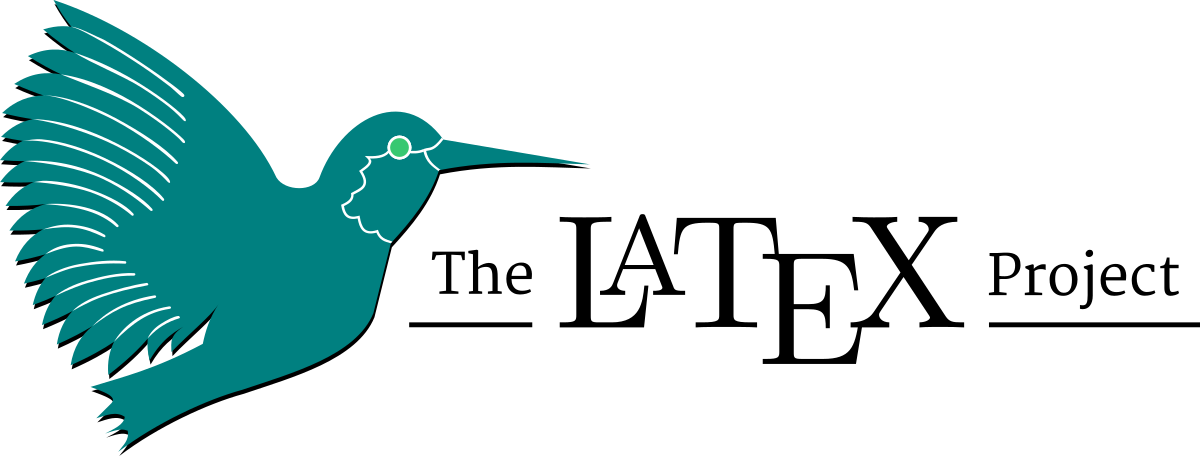
\includegraphics[width=13cm]{figuras/LaTeXproject.png}
	\fonte{\textcite{LaTeX2009}}
	\label{fig:logo}
\end{figure}

\pagebreak
Inserimos a figura \ref{fig:logo} com o seguinte código:

\begin{verbatim}
\begin{figure}[H]
   \centering
   \caption{Logo do projeto \LaTeX.}
   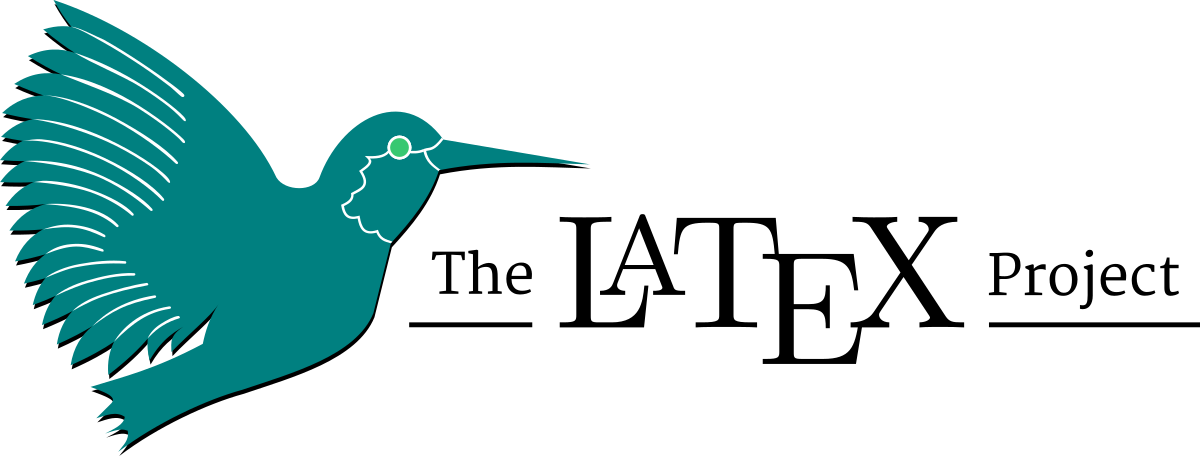
\includegraphics[width=13cm]{figuras/LaTeXproject.png}
   \fonte{\textcite{LaTeX2009}}
   \label{fig:logo}
\end{figure}
\end{verbatim}

No Gráfico \ref{gr:exgrafico} apresentamos um exemplo de gráfico.

\begin{grafico}[H]
\centering
\caption{Evolução de matrículas dos Institutos Federais}
\includegraphics[height=6cm]{./figuras/redefederal.jpg}	
\fonte{MEC/SETEC}
\label{gr:exgrafico}
\end{grafico}

\begin{verbatim}
\begin{grafico}[H]
   \centering
   \caption{Evolução de matrículas dos Institutos Federais}
   \includegraphics[height=6cm]{./figuras/redefederal.jpg}	
   \fonte{MEC/SETEC}
   \label{gr:exgrafico}
\end{grafico}
\end{verbatim}

% Pode-se inserir gráficos diretamente no \LaTeX utilizando-se de pacotes como \verb|pgfplots, tikz|, entre outros. A figura \ref{fig:grafico} ilustra essa possibilidade com o pacote \verb|pgfplots|.

% \begin{grafico}[H]
% \centering
% \caption{Exemplo de gráfico construído no \LaTeX}
% \label{fig:grafico}
%     \begin{tikzpicture}
%     \begin{axis}[hide axis,colormap/cool,]
%     \addplot3[mesh,samples =50,domain = -8:8,]
%     {sin(deg(sqrt(x^2+y^2)))/sqrt(x^2+y^2)};
%     \addlegendentry{$\frac{\sin(r)}{r}$}
%     \end{axis}
%     \end{tikzpicture}
% \fonte{Elaborado pelo autor}
% \end{grafico}

\begin{verbatim}
\begin{grafico}[H]
\centering
\caption{Exemplo de gráfico construído no \LaTeX}
\label{grafico}
    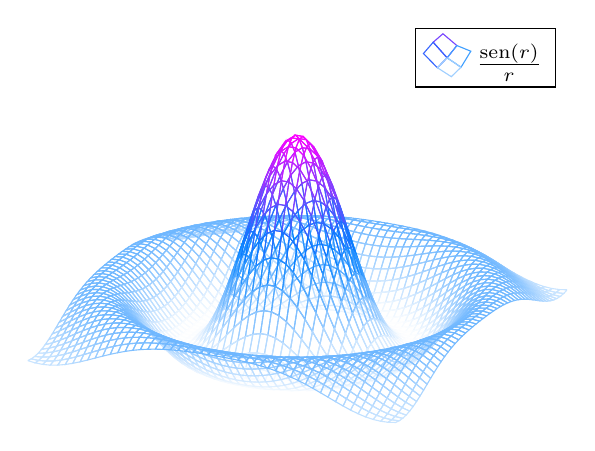
\begin{tikzpicture}
    \begin{axis}[hide axis,colormap/cool,]
    \addplot3[mesh,samples =50,domain = -8:8,]
    {sin(deg(sqrt(x^2+y^2)))/sqrt(x^2+y^2)};
    \addlegendentry{$\frac{\sin(r)}{r}$}
    \end{axis}
    \end{tikzpicture}
\fonte{Elaborado pelo autor}
\end{grafico}
\end{verbatim}

\subsubsection{Tabelas}
As tabelas devem seguir as normas descritas por \textcite{ibge1993}. Sendo formadas por linhas horizontais, devem manter suas bordas laterais abertas e geralmente são utilizadas para dados quantitativos. Os quadros, por outro lado, são formados por linhas verticais e horizontais, devem ter todas suas extremidades fechadas e são mais utilizados para dados qualitativos.

\textcite{abntex2classe} fornece, na classe \verb|abntex2|, a macro \verb|IBGEtab{}{}{}|, que tem por objetivo topo, corpo e rodapé das tabelas com alinhamento conforme descrito em \textcite{ibge1993}. Esta macro deve receber três argumentos para cada uma destas partes da tabela conforme exemplificado na tabela \ref{tab: residentes}. Para representação numérica correta dos dados da tabela, consulte \textcite{ibge1993}.

\pagebreak
\textbf{Exemplo de código para gerar a tabela \ref{tab: residentes} com a macro} \verb|IBGEtab{}{}{}|.

\begin{verbatim}
\begin{table}[H]
\IBGEtab{
   \caption{Pessoas Residentes em domicílios particulares, por sexo e situação do domicílio - Brasil - 1980}%
   \label{tab: residentes}
  }
{
\begin{tabular}{m{2cm}ccc}
   \toprule
   Situação do Total & Total & Mulheres & Homens \\
   \midrule
   Total & 117.960.301 & 59.595.332 & 58.364.969 \\
   Urbana & 79.972.931 & 41.115.439 & 38.857.492 \\
   Rural & 37.987.370 & 18.479.893 & 19.507.477 \\
   \bottomrule
\end{tabular}
}
{
   \fonte{IBGE}
   \nota{Dados fictícios}
}
\end{table}
\end{verbatim}

\begin{table}[H]
\IBGEtab{
  \caption{Pessoas Residentes em domicílios particulares, por sexo e situação do domicílio - Brasil - 1980}%
  \label{tab: residentes}
  }
{
\begin{tabular}{m{2.0cm}ccc}
 \toprule
 Situação do Total & Total & Mulheres & Homens \\
\midrule
Total & 117.960.301 & 59.595.332 & 58.364.969 \\
Urbana & 79.972.931 & 41.115.439 & 38.857.492 \\
Rural & 37.987.370 & 18.479.893 & 19.507.477 \\
\bottomrule
\end{tabular}
}
{
\fonte{IBGE}
\nota{Dados fictícios}
}
\end{table}



\subsection{Quadros}

Os quadros devem ser criados dentro do ambiente \verb|quadro|, podendo sua tabulação ser feita por diversos recursos como os ambientes \verb|tabular, tabularray, tabu, ...|.

Por exemplo, o código abaixo cria o quadro \ref{qua:ex}:

% \begin{lstlisting}[breaklines]
\begin{verbatim}
\begin{quadro}[H]
   \centering
   \caption{Exemplo de quadro simples}
   \label{qua:ex}
   \begin{tabular}{|m{4cm}|m{5cm}|m{3cm}|}
   \hline
   \textbf{Título 1} & \textbf{Título 2} & \textbf{Título 3}\\ \hline
   Texto aqui & Lorem ipsum dolor ...  & Ut accumsan sapien eget magna ... \\ 
   \hline
   Texto da segunda linha & bla bla bla & bla bla bla  \\ \hline
   \end{tabular}
   \fonte{Elaborado pelo autor}
\end{quadro}
\end{verbatim}

\begin{quadro}[H]
   \centering
   \caption{Exemplo de quadro simples}
   \label{qua:ex}
   \begin{tabular}{|m{4cm}|m{5cm}|m{3cm}|}
   \hline
   \textbf{Título 1} & \textbf{Título 2} & \textbf{Título 3}\\ \hline
   Texto aqui & Lorem ipsum dolor ...  & Ut accumsan sapien eget magna ... \\ \hline
   Texto da segunda linha & bla bla bla & bla bla bla  \\ \hline
   \end{tabular}
   \fonte{Elaborado pelo autor}
\end{quadro}

\pagebreak




\section{Exemplo de criação de cronograma}


No caso de projetos de pesquisa, pode ser necessário a criação de um plano de trabalho com a a descrição das etapas do mesmo.

A seguir apresentamos um exemplo de criação feita com algumas customizações do pacote \verb|pgfgantt|.

\begin{verbatim}
%descrição das etapas
\begin{etapas}
    	\item \label{e1} Descrição da etapa 1
    	\item \label{e2} Descrição da etapa 2
    	\item \label{e3} Sed consequat tellus et tortor. Ut tempor laoreet quam.
    	\item \label{e4} Sed consequat tellus et tortor. Ut tempor laoreet quam. 
    	\item \label{e5} Sed consequat tellus et tortor. Ut tempor laoreet quam. 
    	\item \label{e6} Sed consequat tellus et tortor. Ut tempor laoreet quam. 
    	\item \label{e7} Sed consequat tellus et tortor. Ut tempor laoreet quam. 
\end{etapas}

%diagrama com referências às etapas
\begin{center}
        \begin{ganttchart}[vgrid,hgrid]{1}{24}
        \gantttitle{2021}{12} %12 meses em 2021
        \gantttitle{2022}{12} \\ %12 meses em 2022
            \gantttitlelist{1,...,12}{1} % meses 1 ao 12 de 2021
            \gantttitlelist{1,...,12}{1} \\ % meses 1 ao 12 de 2022
                \ganttbar[progress=65]{\ref{e1}}{1}{7} \\
                \ganttbar{\ref{e2}}{7}{12} \\
                \ganttbar{\ref{e3}}{13}{18} \\
                \ganttbar{\ref{e4}}{18}{24}
        \end{ganttchart}
        
        \begin{ganttchart}[vgrid,hgrid]{1}{12}
        \gantttitle{2023}{12}\\ %12 meses em 2023
            \gantttitlelist{1,...,12}{1} \\ % meses 1 ao 12 de 2023
                \ganttbar{\ref{e5}}{1}{7} \\
                \ganttbar{\ref{e6}}{8}{10} \\
                \ganttbar{\ref{e7}}{10}{12}
        \end{ganttchart}
\end{center}
\end{verbatim}


\begin{etapas}
	\item \label{e1} Descrição da etapa 1
	\item \label{e2} Descrição da etapa 2
	\item \label{e3} Sed consequat tellus et tortor. Ut tempor laoreet quam. 
	\item \label{e4} Sed consequat tellus et tortor. Ut tempor laoreet quam. 
	\item \label{e5} Sed consequat tellus et tortor. Ut tempor laoreet quam. 
	\item \label{e6} Sed consequat tellus et tortor. Ut tempor laoreet quam. 
	\item \label{e7} Sed consequat tellus et tortor. Ut tempor laoreet quam. 
\end{etapas}

\begin{center}

\begin{ganttchart}[vgrid,hgrid]{1}{24}
\gantttitle{2021}{12} %12 meses em 2021
\gantttitle{2022}{12} \\ %12 meses em 2022
    \gantttitlelist{1,...,12}{1} % meses 1 ao 12 de 2021
    \gantttitlelist{1,...,12}{1} \\ % meses 1 ao 12 de 2022
        \ganttbar[progress=65]{\ref{e1}}{1}{7} \\
        \ganttbar{\ref{e2}}{7}{12} \\
        \ganttbar{\ref{e3}}{13}{18} \\
        \ganttbar{\ref{e4}}{18}{24}
\end{ganttchart}

\begin{ganttchart}[vgrid,hgrid]{1}{12}
\gantttitle{2023}{12}\\ %12 meses em 2023
    \gantttitlelist{1,...,12}{1} \\ % meses 1 ao 12 de 2023
        \ganttbar{\ref{e5}}{1}{7} \\
        \ganttbar{\ref{e6}}{8}{10} \\
        \ganttbar{\ref{e7}}{10}{12}
\end{ganttchart}

\end{center}
\include{capitulos/conclusao}             % Conclusão

%-----------------------
% ELEMENTOS PÓS-TEXTUAIS %
%-----------------------
    \postextual
    \printbibliography
    % \bibliography{./refbase}    % Geração automática das referências por meio do arquivo 'refbase.bib'
    % \printbibliography % Geração automática das referências por meio do arquivo 'refbase.bib'
    \include{elementos-pos-textuais/apendices}   % Apêndices
    \include{elementos-pos-textuais/anexos}  % Anexos
  
    \printindex  % Imprimie o índice remissivo
\end{document}
